\documentclass{standalone}
\usepackage{ tikz }
\usetikzlibrary{shapes}
\usetikzlibrary{plotmarks}
\usepackage{ xparse }
\usepackage{../../../macros}

\begin{document}
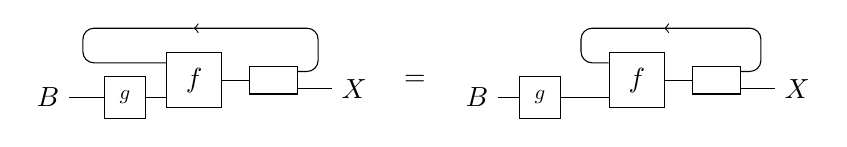
\begin{tikzpicture}[yscale=-1,x=1em,y=1.25em]
        
    \draw (-2.5,0) -- (-1.25,0);
    \draw (0.25,0) -- (1,0);
    \node[draw, minimum height = 2em, minimum width = 2em, anchor = west] at (1,-0.5){$f$};
    \node[draw, minimum height = 1.5em, minimum width = 1.5em, anchor = west] at (-1.25, 0){\scalebox{0.75}{$g$}};
    \draw (3,-0.5) -- (4,-0.5);
    \node[draw, minimum height = 1em, minimum width = 1.75em, anchor = west] at (4,-0.5){$\ccopy{}$};
    \draw [rounded corners, ->] (5.75,-0.75) -- (6.5, -0.75) -- (6.5,-2) -- (2, -2);
    \draw [rounded corners] (2,-2) -- (-2,-2) -- (-2,-1) -- (1,-1);
    \draw [rounded corners] (5.75,-0.25) -- (7,-0.25);

    \node [anchor=east] at (-2.5,0) {$B$};
    \node [anchor=west] at (7,-0.25) {$X$};

    \node at (10,-0.5) {$=$};

    \node [anchor=east] at (13,0) {$B$};
    \draw (13,0) -- (13.75,0);
    \node[draw, minimum height = 1.5em, minimum width = 1.5em, anchor = west] at (13.75, 0){\scalebox{0.75}{$g$}};
    \draw (15.25, 0) -- (17,0);
    \node[draw, minimum height = 2em, minimum width = 2em, anchor = west] at (17,-0.5){$f$};
    \draw (19,-0.5) -- (20,-0.5);
    \node[draw, minimum height = 1em, minimum width = 1.75em, anchor = west] at (20,-0.5){$\ccopy{}$};
    \draw [rounded corners, ->] (21.75,-0.75) -- (22.5, -0.75) -- (22.5,-2) -- (19, -2);
    \draw [rounded corners] (19,-2) -- (16,-2) -- (16,-1) -- (17,-1);
    \draw (21.75,-0.25) -- (23,-0.25);
    \node [anchor=west] at (23,-0.25) {$X$};

\end{tikzpicture}
\end{document}